\documentclass{article}
\usepackage[utf8]{inputenc}
\usepackage{listings}
\usepackage{multimedia} % to embed movies in the PDF file
\usepackage{graphicx}
\usepackage{comment}
\usepackage[english]{babel}
\usepackage{amsmath}
\usepackage{amsfonts}
\usepackage{subfigure}
\usepackage{wrapfig}
\usepackage{multirow}
\usepackage{verbatim}

\newtheorem{theorem}{Theorem}[section]
\newtheorem{lemma}[theorem]{Lemma}
\newtheorem{corollary}[theorem]{Corollary}
%\newtheorem{algorithm}[theorem]{Algorithm}
\newtheorem{remark}[theorem]{Remark}
\newenvironment{proof}{\noindent {\bf Proof:} }{\hfill $\Box$ \\[2ex] }
\newenvironment{keywords}{\begin{quote} {\bf Key words} }
                         {\end{quote} }
\newenvironment{AMS}{\begin{quote} {\bf AMS subject classifications} }
                         {\end{quote} }


\newcommand{\eref}[1]{\mbox{\rm(\ref{#1})}}
\newcommand{\tref}[1]{\mbox{\rm\ref{#1}}}
\newcommand{\set}[2]{\left\{ #1 \; : \; #2 \right\} }
\newcommand{\deq}{\raisebox{0pt}[1ex][0pt]{$\stackrel{\scriptscriptstyle{\rm def}}{{}={}}$}}

\newcommand {\DS} {\displaystyle}

\newcommand{\real}{\mathbb{R}}
\newcommand{\compl}{\mathbb{C}}



\newcommand {\half} {\mbox{$\frac{1}{2}$}}
\newcommand{\force}{{\mathbf{f}}}
\newcommand{\strain}{{\boldsymbol{\varepsilon}}}
\newcommand{\stress}{{\boldsymbol{\sigma}}}
\renewcommand{\div}{{\boldsymbol{\nabla}}}

\newcommand {\cA} {{\cal A}}
\newcommand {\cB} {{\cal B}}
\newcommand {\cC} {{\cal C}}
\newcommand {\cD} {{\cal D}}
\newcommand {\cE} {{\cal E}}
\newcommand {\cL} {{\cal L}}
\newcommand {\cP} {{\cal P}}
\newcommand {\cQ} {{\cal Q}}
\newcommand {\cR} {{\cal R}}
\newcommand {\cV} {{\cal V}}
\newcommand {\cW} {{\cal W}}
\newcommand {\CH} {{\cal H}}
\newcommand {\CS} {{\cal S}}


\newcommand{\bzero}{\mathbf{0}}
\newcommand{\ba}{\mathbf{a}}
\newcommand{\bb}{\mathbf{b}}
\newcommand{\bc}{\mathbf{c}}
\newcommand{\bd}{\mathbf{d}}
\newcommand{\be}{\mathbf{e}}
\newcommand{\bff}{\mathbf{f}}
\newcommand{\bg}{\mathbf{g}}
\newcommand{\bh}{\mathbf{h}}
\newcommand{\bn}{\mathbf{n}}
\newcommand{\bp}{\mathbf{p}}
\newcommand{\bq}{\mathbf{q}}
\newcommand{\br}{\mathbf{r}}
\newcommand{\bs}{\mathbf{s}}
\newcommand{\bt}{\mathbf{t}}
\newcommand{\bu}{\mathbf{u}}
\newcommand{\bv}{\mathbf{v}}
\newcommand{\bw}{\mathbf{w}}
\newcommand{\bx}{\mathbf{x}}
\newcommand{\by}{\mathbf{y}}
\newcommand{\bz}{\mathbf{z}}
\newcommand{\bA}{\mathbf{A}}
\newcommand{\bB}{\mathbf{B}}
\newcommand{\bC}{\mathbf{C}}
\newcommand{\bD}{\mathbf{D}}
\newcommand{\bE}{\mathbf{E}}
\newcommand{\bF}{\mathbf{F}}
\newcommand{\bG}{\mathbf{G}}
\newcommand{\bH}{\mathbf{H}}
\newcommand{\bI}{\mathbf{I}}
\newcommand{\bJ}{\mathbf{J}}
\newcommand{\bK}{\mathbf{K}}
\newcommand{\bL}{\mathbf{L}}
\newcommand{\bM}{\mathbf{M}}
\newcommand{\bN}{\mathbf{N}}
\newcommand{\bO}{\mathbf{O}}
\newcommand{\bP}{\mathbf{P}}
\newcommand{\bQ}{\mathbf{Q}}
\newcommand{\bR}{\mathbf{R}}
\newcommand{\bS}{\mathbf{S}}
\newcommand{\bU}{\mathbf{U}}
\newcommand{\bV}{\mathbf{V}}
\newcommand{\bW}{\mathbf{W}}
\newcommand{\bX}{\mathbf{X}}
\newcommand{\bY}{\mathbf{Y}}
\newcommand{\bZ}{\mathbf{Z}}

\newcommand{\cO}{ {\cal O} }
\newcommand{\CT}{ {\cal T} }
\newcommand{\IL}{{\mathbb L}}
\newcommand{\sIL}{{{{\mathbb L}_s}}}
\newcommand{\bOmega}{{\boldsymbol{\Omega}}}
\newcommand{\bPsi}{{\boldsymbol{\Psi}}}

\newcommand{\bgamma}{{\boldsymbol{\gamma}}}
\newcommand{\bmu}{{\boldsymbol{\mu}}}
\newcommand{\blambda}{{\boldsymbol{\lambda}}}
\newcommand{\bLambda}{{\boldsymbol{\Lambda}}}
\newcommand{\bpi}{{\boldsymbol{\pi}}}
\newcommand{\bPi}{{\boldsymbol{\Pi}}}
\newcommand{\bphi}{{\boldsymbol{\phi}}}
\newcommand{\bPhi}{{\boldsymbol{\Phi}}}
\newcommand{\bpsi}{{\boldsymbol{\psi}}}
\newcommand{\btheta}{{\boldsymbol{\theta}}}
\newcommand{\bTheta}{{\boldsymbol{\Theta}}}
\newcommand{\bSigma}{{\boldsymbol{\Sigma}}}
\newcommand{\sump}{\sideset{}{^{'}}\sum} 
\DeclareMathOperator*{\Res}{Res}
\DeclareMathOperator{\OO}{O}
\DeclareMathOperator{\oo}{o}
\DeclareMathOperator{\erfc}{erfc}
\def\Xint#1{\mathchoice
   {\XXint\displaystyle\textstyle{#1}}%
   {\XXint\textstyle\scriptstyle{#1}}%
   {\XXint\scriptstyle\scriptscriptstyle{#1}}%
   {\XXint\scriptscriptstyle\scriptscriptstyle{#1}}%
   \!\int}
\def\XXint#1#2#3{{\setbox0=\hbox{$#1{#2#3}{\int}$}
     \vcenter{\hbox{$#2#3$}}\kern-.5\wd0}}
\def\ddashint{\Xint=}
\def\pvint{\Xint-}






\title{AMATH 568 Homework 4}
\author{Cade Ballew \#2120804}
\date{February 2, 2022}

\begin{document}
	
\maketitle
	
\section{Problem 1}
Consider \begin{align*}
    \mathrm{AI}(x) = \frac{1}{2 \pi i} \int_C e^{i z x + i z^3/3} \frac{d z}{z}, \quad x \in \mathbb R,
  \end{align*}
  as $x \to \pm \infty$ where $C$ is a contour in the upper-half of the complex $z$-plane described by
  \begin{align*}
    C = \{ u(s) : s \in \mathbb R\},
  \end{align*}
  for a sufficiently nice function $u$, oriented in the direction of increasing $s$ where
  \begin{align*}
  \lim_{s \to \pm \infty} |u(s)| = \infty, \quad   \lim_{s \to + \infty} \frac{u(s)}{|u(s)|} = e^{i \pi/6}, \quad \lim_{s \to - \infty} \frac{u(s)}{|u(s)|} = e^{i 5\pi/6}.
  \end{align*}
We first let $x=\sigma|x|$ where $\sigma=\pm1$ so that we can consider $x \to \pm \infty$ by considering two cases based on $\sigma$. Then,
\[
\mathrm{AI}(x) = \frac{1}{2 \pi i} \int_C e^{i z |x|\sigma + i z^3/3} \frac{d z}{z}.
\]
Now, consider the change of variables $z=u|x|^a$ for some constant $a$. Then,
\[
e^{i z |x|\sigma + i z^3/3}=e^{iu|x|^{1+a}\sigma+iu^3u^3|x|^{3a}/3},
\]
so in order to be able to factor out all the $|x|$ terms, we need that $3a=1+a$, i.e. that $a=1/2$. If we consider this change of variables $z=u|x|^{1/2}$, then
\[
\mathrm{AI}(x) = \frac{1}{2 \pi i} \int_C e^{i  u|x|^{3/2}\sigma + i u^3|x|^{3/2}/3} \frac{|x|^{1/2}du}{u|x|^{1/2}}.
\]
Renaming $u$ to $z$ for simplicity, we have that 
\[
\mathrm{AI}(x) = \frac{1}{2 \pi i} \int_C e^{  |x|^{3/2}(iz\sigma + iz^3/3)} \frac{dz}{z}=\frac{1}{2 \pi i} \int_C e^{|x|^{3/2}h(z)}g(z)dz
\]
where $h(z)=iz\sigma + iz^3/3$ and $g(z)=1/z$. Note that $h(z)$ is entire for either value of $\sigma$ and that $g(z)$ is analytic except at $z=0$, so we can apply the method of steepest descent as $|x|\to\infty$ with potential issues only at $z=0$. \\
First, we consider the case where $\sigma=1$ which corresponds with $x\to\infty$. Then, $h(z)=iz+iz^3/3$, so $0=h'(z)=i+iz^2$ when $z=\pm i$, so our saddle points are $z_1=i$ and $z_2=-i$. We also note that $h''(z)=2iz$, so $h''(z_1)=-2\neq0$ and $h''(z_2)=2\neq0$. Now, we investigate the real and imaginary parts of $h$ which are given by 
\[
R(x,y)=-y-x^2y+\frac{y^3}{3}
\]
and 
\[
I(x,y)=x+\frac{x^3}{3}-xy^2
\]
if $z=x+iy$. We wish to find a path to which we may deform our contour $C$ where $I(x,y)$ is constant. A reasonable choice seems to be the level curve that passes through our saddle point at $z_1=i$, since ideally, we will not need to deform into the lower half plane to avoid the singularity at $z=0$. We have that $h(z_1)=-2/3$, so in order to keep $I(x,y)$ constant, we need to consider where $I(x,y)=0$. $I(x,y)=x(1+x^2/3-y^2)$, so this is true either where $x=0$ or $1+x^2/3-y^2=0$ and we consider the latter. This is a hyperbola in both the upper and lower half planes, so we also restrict it to the upper half plane to match our desired angles. Thus, we consider 
\[
C=\{u(s)=x+iy\in\mathbb{C} ~|~s\in\real,~ y\geq0, ~ 1+x^2/3-y^2=0\}.
\]
The following figure shows $C$ drawn on a contour plot of $I(x,y)$.\\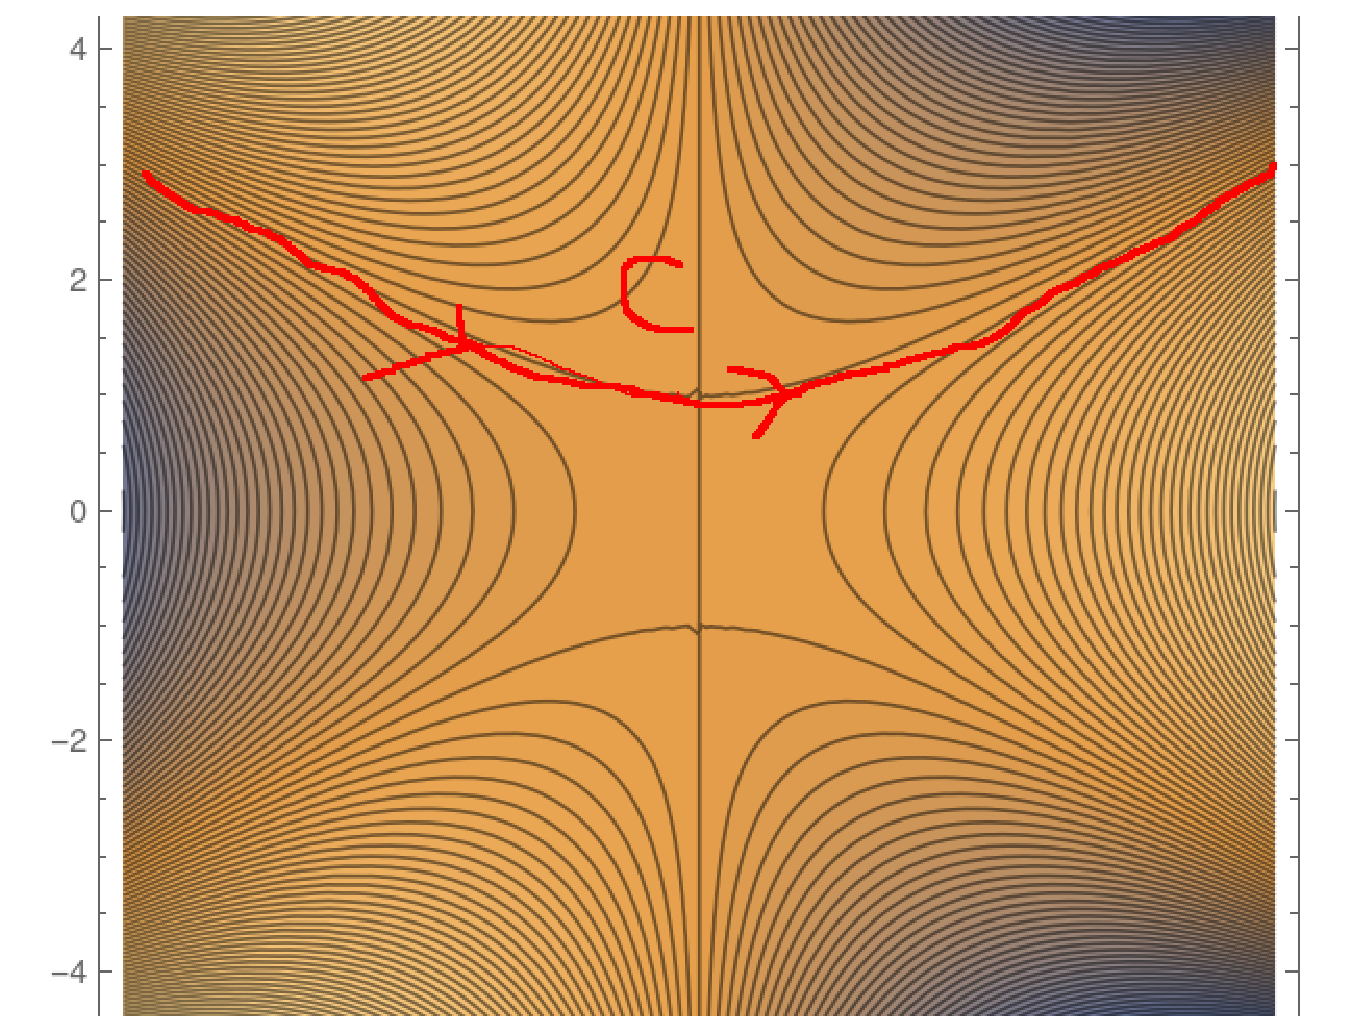
\includegraphics[scale=0.4]{568hw4fig1.eps}\\
Now, we wish to evaluate the large $z$ behavior for $C$ to ensure that our contour goes to infinity in the proper direction. Substituting $z=re^{i\theta}$ into $1+x^2/3-y^2=0$, we have that $1+r^2\cos^2\theta/3-r^2\sin^2\theta=0$ which we can rewrite as 
\[
\frac{3}{r^2}+\cos^2\theta-3\sin^2\theta=0
\]
since we are considering $r\to\infty$. Now, we can let $\epsilon=1/r$ and 
\[
0=f(\theta,\epsilon)=\cos^2\theta-3\sin^2\theta+\OO(\epsilon^2)=-4\sin^2\theta+1+\OO(\epsilon^2).
\]
Solving $f(\theta,0)=0$, we find that $\sin\theta=\pm1/2$, so $\theta=\pi/6,5\pi/6,7\pi/6,13\pi/6$, but our contour also has the restriction that $\Im(z)\geq0$, so we only consider $\theta_k=\pi/6,5\pi/6$. Now, to be completely rigorous, we can note that $\frac{\partial f}{\partial\theta}\neq0$ at these values of $\theta_k$ and apply the IFT to determine that $\theta(\epsilon)=\theta_k+\OO(\epsilon^2)=\theta_k+\OO(1/r^2)$ as $r\to\infty$. Thus, we observe that our contour goes to $\infty$ at the proper angles. 
%maybe argue specific angles somehow 
\\
Since we know that the imaginary part of $h$ is zero on our new contour $C$, we can look just at the real part on our contour. As $z\to\infty$, $z=re^{i\pi/6}$ or $z=re^{5i\pi/6}$ as $r\to\infty$. In either case, the $iz^3/3$ term dominates $h(z)$ and is given by $ir^3e^{i\pi/2}/3=-r^3/3$, the real part of $h$ looks like $-r^3/3$ as $z\to\infty$ on our contour which tends to $-\infty$ and will be decay in an exponential. The only saddle point $z_1=i$ on our contour has $R(x_1,y_1)=-2/3$ which gives the dominant contribution. From this, define $\Tilde{h}(z)=h(z)-h(z_1)=h(z)+2/3$ and write
\[
\mathrm{AI}(x)=\frac{1}{2 \pi i} \int_C e^{|x|^{3/2}h(z)}g(z)dz=\frac{1}{2 \pi i} e^{-2|x|^{3/2}/3}\int_C e^{|x|^{3/2}\Tilde{h}(z)}g(z)dz.
\]
Now, we attempt to localize our contour around our saddle point. Considering the parameterization of our contour, adopt the convention $u(s^*)=z_1$ and consider $s_-<s^*<s_+$ to be a sufficiently small neighborhood around $s^*$ and let $u(s_-)=z_-$ and $u(s_+)=z_+$. We split our contour $C=C_1+C_2+C_3$ where $C_1$ is the contour from infinity at the left to $z_-$, $C_2$ is the contour from $z_-$ to $z_+$, and $C_3$ is the contour from $z_+$ to infinity on the right. Now, we bound
\begin{align*}
\int_{C_1}e^{|x|^{3/2}\Tilde{h}(z)}g(z)dz&=e^{|x|^{3/2}\Tilde{h}(z_-)}\int_{C_1}e^{|x|^{3/2}\overbrace{(\Tilde{h}(z)-\Tilde{h}(z_-))}^{\text{negative}}}g(z)dz\\&\leq
e^{|x|^{3/2}\Tilde{h}(z_-)}\underbrace{\int_{C_1}e^{|x|^{3/2}(\Tilde{h}(z)-\Tilde{h}(z_-))}|g(z)||dz|}_{\text{finite}}
\end{align*}
which is beyond all orders as $|x|\to\infty$. Similarly,
\begin{align*}
\int_{C_3}e^{|x|^{3/2}\Tilde{h}(z)}g(z)dz&=e^{|x|^{3/2}\Tilde{h}(z_+)}\int_{C_3}e^{|x|^{3/2}\overbrace{(\Tilde{h}(z)-\Tilde{h}(z_+))}^{\text{negative}}}g(z)dz\\&\leq
e^{|x|^{3/2}\Tilde{h}(z_+)}\underbrace{\int_{C_3}e^{|x|^{3/2}(\Tilde{h}(z)-\Tilde{h}(z_+))}|g(z)||dz|}_{\text{finite}}
\end{align*}
is also beyond all orders as $|x|\to\infty$. Thus, we can localize our contour to $C_2$ at the cost of a BAO error. \\
Now that we have localized, we consider the behavior in a neighborhood around our saddle point by applying a change of variables with the IFT. Namely, we consider 
\[
\frac{\Tilde{h}(z_1+s\phi)}{s^2}+1=0.
\]
Now, we can simply apply the formula on page 108 of the text to get that
\begin{align*}
\int_{C_2}e^{|x|^{3/2}h(z)}g(z)dz&={|x|^{3/2}}^{-1/2}e^{-2|x|^{3/2}/3}\left(e^{i\theta(z_1)}\sqrt{\frac{2\pi}{|h''(z_1)|}}g(z_1)+\OO(|x|^{-3/2})\right)
\end{align*}
where $\theta(z_1)$ is the angle at which $C$ leaves $z_1$. We can see from our change of variables that this is given by the angle of $\phi(0)$, so we compute 
\[
\phi(0)=\pm\sqrt{\frac{-2}{h''(z_1)}}=\pm1.
\]
Thus, we enter/leave at angles of $\theta=0,\pi$, and $\theta(z_1)=0$ with our convention. With this, we can write 
\begin{align*}
\mathrm{AI}(x)&=\frac{1}{2\pi i}|x|^{-3/4}e^{-2|x|^{3/2}/3}\left(\sqrt{\pi}\frac{1}{i}+\OO(|x|^{-3/2})\right)\\&=
-\frac{1}{2\sqrt{\pi}}e^{-2|x|^{3/2}/3}(|x|^{-3/4}+\OO(|x|^{-9/4}))+\text{BAO}
\end{align*}
as $x\to\infty$.\\
\break
Now, consider the case where $x\to-\infty$, i.e. that $\sigma=-1$ so that $h(z)=-iz+iz^3/3$ and $0=h'(z)=-i+iz^2$ when $z=\pm1$; take our saddle points to be $z_1=-1$, $z_2=1$. Also note that $h''(z)=2iz$, so $h''(z_1)=-2i\neq0$ and $h''(z_2)=2i\neq0$. Now, we investigate the real and imaginary parts of $h$ which are 
\[
R(x,y)=y-x^2y+\frac{y^3}{3}
\]
and
\[
I(x,y)=-x+\frac{x^3}{3}-xy^2.
\]
To go about deforming our contour, we look to choose a new contour that passes through our saddle points with constant imaginary part. At $z=1$, $h(z)=-2i/3$ and at $z=-1$, $h(z)=2i/3$. Thus, we consider
\[
C_1=\{u(s)=x+iy\in\mathbb{C} ~|~s\in\real,~ x\leq0, ~ -x+\frac{x^3}{3}-xy^2=2/3\}. 
\]
This set actually includes two separate curves, so we will abuse notation and adopt the convention that $C_1$ only refers to the curve for which $y$ decreases as $x$ increases. The following figure shows $C_1$ drawn on a contour plot of $I(x,y)$.\\
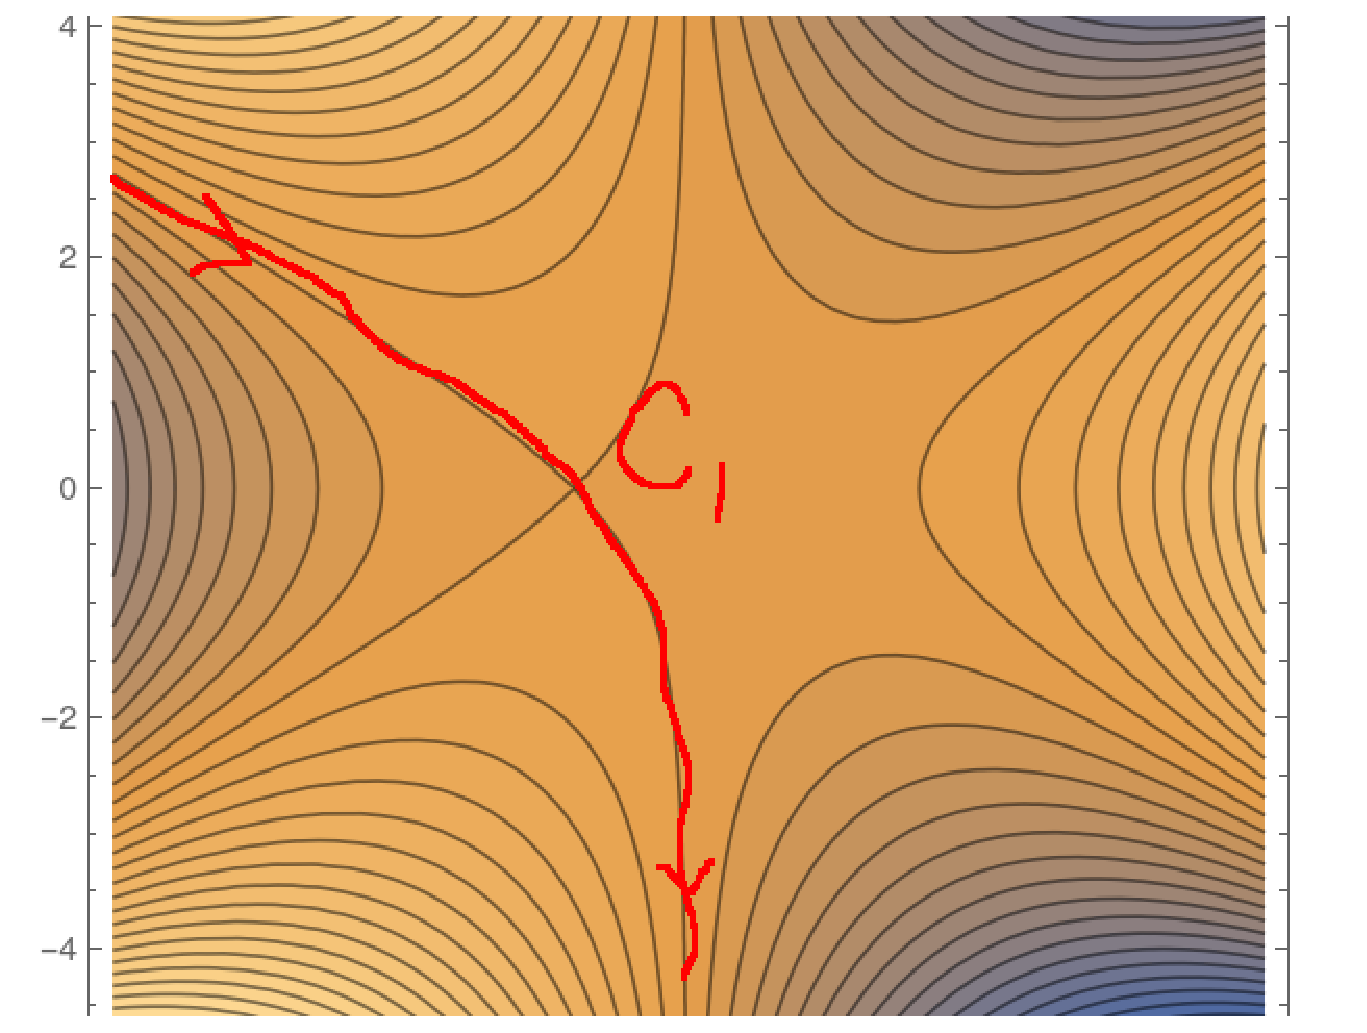
\includegraphics[scale=0.4]{568hw4fig2.eps}\\
We also consider
\[
C_2=\{u(s)=x+iy\in\mathbb{C} ~|~s\in\real,~ x\geq0, ~ -x+\frac{x^3}{3}-xy^2=-2/3\}
\]
where we again abuse notation and say that this curve is increasing in $y$ when it is increasing in $x$. The following figure shows $C_2$ drawn on a contour plot of $I(x,y)$.\\
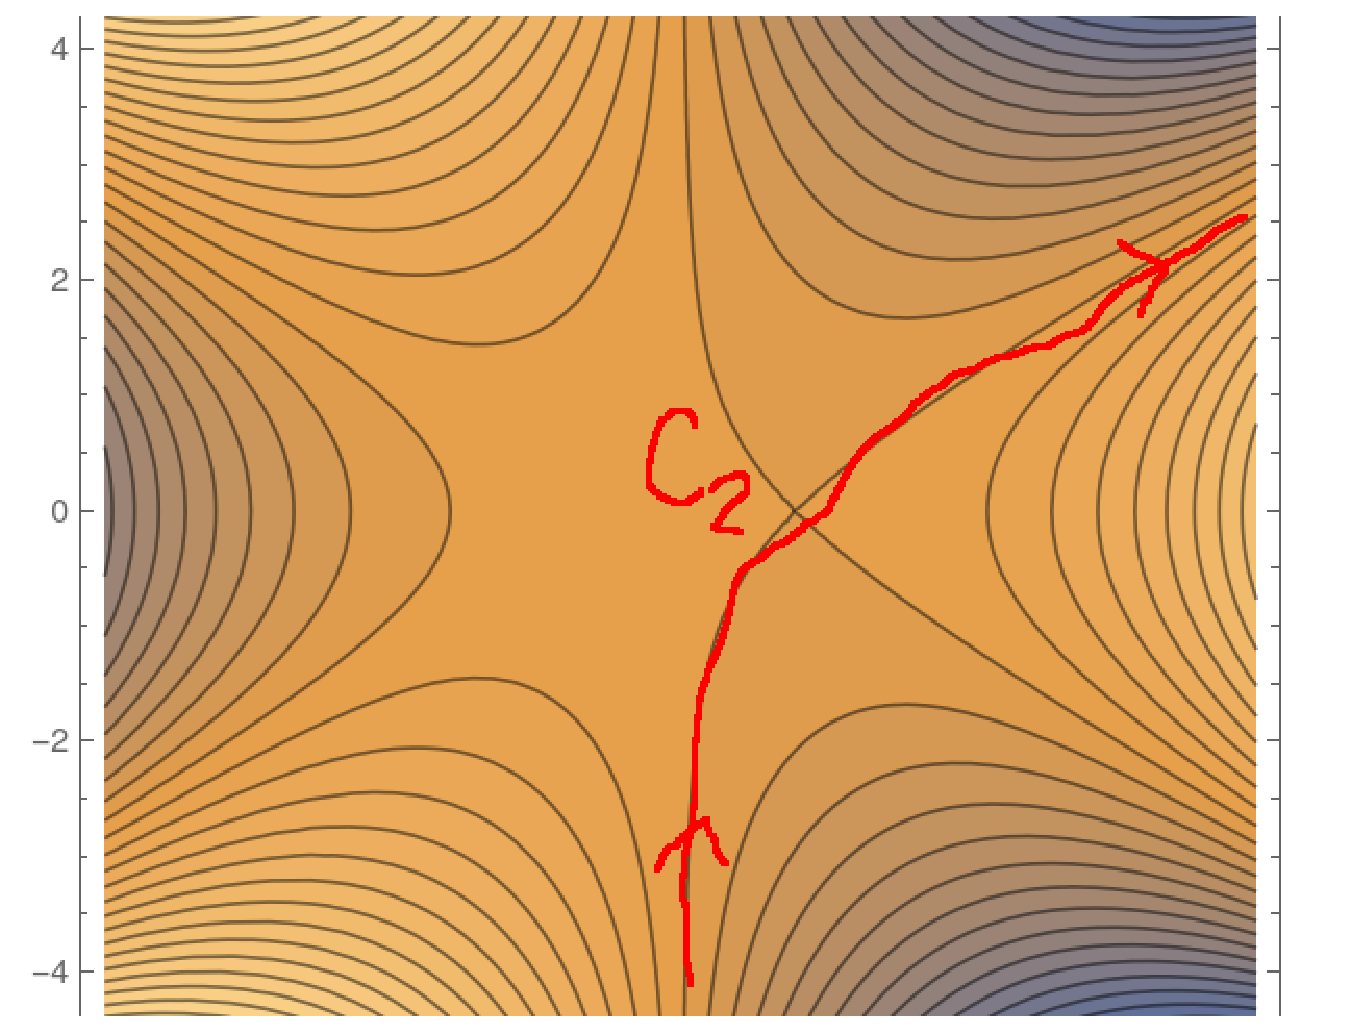
\includegraphics[scale=0.4]{568hw4fig3.eps}\\
Now, we compute 
\[
\Res_{z=0}e^{|x|^{3/2}h(z)}g(z)=\Res_{z=0}\frac{e^{|x|^{3/2}(-iz+iz^3/3)}}{z}=\lim_{z\to0}e^{|x|^{3/2}(-iz+iz^3/3)}=1.
\]
Applying the residue theorem to deform our contour, 
\[
\frac{1}{2 \pi i} \int_{-C} e^{|x|^{3/2}h(z)}g(z)dz+\frac{1}{2 \pi i} \int_{C_1} e^{|x|^{3/2}h(z)}g(z)dz+\frac{1}{2 \pi i} \int_{C_2} e^{|x|^{3/2}h(z)}g(z)dz=\Res_{z=0}e^{|x|^{3/2}h(z)}g(z),
\]
so
\[
\frac{1}{2 \pi i} \int_{C} e^{|x|^{3/2}h(z)}g(z)dz=\frac{1}{2 \pi i} \int_{C_1} e^{|x|^{3/2}h(z)}g(z)dz+\frac{1}{2 \pi i} \int_{C_2} e^{|x|^{3/2}h(z)}g(z)dz-1.
\]
We do need to confirm that this is a valid deformation by showing that $C_1$ and $C_2$ go off to infinity at the correct angles. To do this, we substitute $z=re^{i\theta}$ into $-x+x^3/3-xy^2=2/3$, we have that $-r\cos\theta+r^3\cos^3\theta/3-r^3\cos\theta\sin^2\theta=2/3$ which we can rewrite as 
\[
-\frac{2}{r^3}+\cos\theta\left(-\frac{3}{r^2}+\cos^2\theta-3\sin^2\theta\right)=0
\]
since we are considering $r\to\infty$. Now, we can let $\epsilon=1/r$ and 
\[
0=f(\theta,\epsilon)=\cos\theta(\cos^2\theta-3\sin^2\theta)+\OO(\epsilon^2)=\cos\theta(-4\sin^2\theta+1)+\OO(\epsilon^2).
\]
Solving $f(\theta,0)=0$, we find that either $\sin\theta=\pm1/2$, so $\theta=\pi/6,5\pi/6,7\pi/6,13\pi/6$ or $\cos\theta=0$, so $\theta=\pi/2,3\pi/2$. Our contour also has the restriction that $\Re(z)\leq0$, so we only consider $\theta_k=\pi/2,5\pi/6,7\pi/6,3\pi/2$. Now, to be completely rigorous, we can note that $\frac{\partial f}{\partial\theta}\neq0$ at these values of $\theta_k$ and apply the IFT to determine that $\theta(\epsilon)=\theta_k +\OO(\epsilon^2)=\theta_k+\OO(1/r^2)$ as $r\to\infty$. If we plot the two curves associated with this region, we can see that one goes to $\infty$ above the real axis and along the imaginary axis in the lower half plane. This is the curve that we have chosen, so clearly it goes to zero at $\theta_k=5\pi/6,3\pi/2$ as desired. Similarly, if we consider $-x+x^3/3-xy^2=-2/3$, we essentially have the same $f(\theta,\epsilon)$ since the only term that changes is absorbed into the $\OO(\epsilon^2)$ term. However, we now consider $\Re(z)\geq0$, so we instead have $\theta_k=\pi/6,\pi/2,3\pi/2,13\pi/6$. Again, we pick the curve that goes to $\infty$ along the imaginary axis in the lower half plane and above the real axis. Thus, our deformation is valid. \\
First consider the contour $C_1$. As $z\to\infty$, $z=re^{3i\pi/2}$ or $z=re^{5i\pi/6}$ as $r\to\infty$. In either case, the $iz^3/3$ term dominates $h(z)$ and is given by $ir^3e^{i\pi/2}/3=-r^3/3$, the real part of $h$ looks like $-r^3/3$ as $z\to\infty$ on our contour which goes to $-\infty$ as $r\to\infty$, giving decay when in an exponential. Similarly, we can see that this is true on the contour $C_2$ as well, because as $z\to\infty$, $z=re^{3i\pi/2}$ or $z=re^{i\pi/6}$ as $r\to\infty$. In either case, the $iz^3/3$ term dominates $h(z)$ and is given by $ir^3e^{i\pi/2}/3=-r^3/3$, the real part of which also looks like $-r^3/3$. Now, we compute $h(z_1)=2i/3$ and $h(z_2)=-2i/3$ and define $h_1(z)=h(z)-h(z_1)=h(z)-2i/3$ and $h_2(z)=h(z)-h(z_2)=h(z)+2i/3$. We can see two equal "dominant" contributions, so we will seek to localize around each saddle point. Now, we write
\[
\mathrm{AI}(x)=\frac{1}{2 \pi i} e^{2i|x|^{3/2}/3}\int_{C_1} e^{|x|^{3/2}h_1(z)}g(z)dz+\frac{1}{2 \pi i} e^{-2i|x|^{3/2}/3}\int_{C_2} e^{|x|^{3/2}h_2(z)}g(z)dz-1.
\]
First for $C_1$, considering the parameterization of our contour, adopt the convention $u(s^*)=z_1$ and consider $s_-<s^*<s_+$ be a sufficiently small neighborhood around $s^*$ and let $u(s_-)=z_-$ and $u(s_+)=z_+$. We split our contour $C_1=C_{1a}+C_{1b}+C_{1c}$ where $C_{1a}$ is the contour from infinity at the left to $z_-$, $C_{1b}$ is the contour from $z_-$ to $z_+$, and $C_{1c}$ is the contour from $z_+$ to infinity on the right. Now, we bound
\begin{align*}
\int_{C_{1a}}e^{|x|^{3/2}h_1(z)}g(z)dz&=e^{|x|^{3/2}h_1(z_-)}\int_{C_{1a}}e^{|x|^{3/2}\overbrace{(h_1(z)-h_1(z_-))}^{\text{negative}}}g(z)dz\\&\leq
e^{|x|^{3/2}h_1(z_-)}\underbrace{\int_{C_{1a}}e^{|x|^{3/2}(h_1(z)-h_1(z_-))}|g(z)||dz|}_{\text{finite}}
\end{align*}
which is beyond all orders as $|x|\to\infty$. Similarly,
\begin{align*}
\int_{C_{1c}}e^{|x|^{3/2}h_1(z)}g(z)dz&=e^{|x|^{3/2}h_1(z_+)}\int_{C_{1c}}e^{|x|^{3/2}\overbrace{(h_1(z)-h_1(z_+))}^{\text{negative}}}g(z)dz\\&\leq
e^{|x|^{3/2}h_1(z_+)}\underbrace{\int_{C_{1c}}e^{|x|^{3/2}(h_1(z)-h_1(z_+))}|g(z)||dz|}_{\text{finite}}
\end{align*}
is also beyond all orders as $|x|\to\infty$. Thus, we can localize $C_1$ to $C_{1b}$ at the cost of a BAO error. We can make the same argument for $C_2$. Namely, if we reuse the convention (these variables have the same names but are obviously different from the $C_1$ case) $u(s^*)=z_1$ and consider $s_-<s^*<s_+$ be a sufficiently small neighborhood around $s^*$ and let $u(s_-)=z_-$ and $u(s_+)=z_+$. We split our contour $C_2=C_{2a}+C_{2b}+C_{2c}$ where $C_{2a}$ is the contour from infinity at the left to $z_-$, $C_{2b}$ is the contour from $z_-$ to $z_+$, and $C_{2c}$ is the contour from $z_+$ to infinity on the right. Now, we bound
\begin{align*}
\int_{C_{2a}}e^{|x|^{3/2}h_2(z)}g(z)dz&=e^{|x|^{3/2}h_2(z_-)}\int_{C_{2a}}e^{|x|^{3/2}\overbrace{(h_2(z)-h_2(z_-))}^{\text{negative}}}g(z)dz\\&\leq
e^{|x|^{3/2}h_2(z_-)}\underbrace{\int_{C_{2a}}e^{|x|^{3/2}(h_2(z)-h_2(z_-))}|g(z)||dz|}_{\text{finite}}
\end{align*}
which is beyond all orders as $|x|\to\infty$. Similarly,
\begin{align*}
\int_{C_{2c}}e^{|x|^{3/2}h_2(z)}g(z)dz&=e^{|x|^{3/2}h_2(z_+)}\int_{C_{2c}}e^{|x|^{3/2}\overbrace{(h_2(z)-h_2(z_+))}^{\text{negative}}}g(z)dz\\&\leq
e^{|x|^{3/2}h_2(z_+)}\underbrace{\int_{C_{2c}}e^{|x|^{3/2}(h_2(z)-h_2(z_+))}|g(z)||dz|}_{\text{finite}}
\end{align*}
is also beyond all orders as $|x|\to\infty$. Thus, we can localize $C_2$ to $C_{2b}$ at the cost of a BAO error.\\
Now that we have localized, let us first consider the behavior in a neighborhood around $z_1$ by applying a change of variables with the IFT. Namely, we consider 
\[
\frac{h_1(z_1+s\phi)}{s^2}+1=0.
\]
Now, we apply the formula on page 108 of the text to get that 
\[
\int_{C_{1b}}e^{|x|^{3/2}h(z)}g(z)dz={|x|^{3/2}}^{-1/2}\left(e^{i\theta(z_1)}\sqrt{\frac{2\pi}{|h''(z_1)|}}g(z_1)+\OO(|x|^{-3/2})\right)
\]
with $\theta(z_1)$ defined in the same way as before. We compute
\[
\phi(0)=\pm\sqrt{\frac{-2}{h''(z_1)}}=\pm\sqrt{-i}=\pm e^{-i\pi/4}.
\]
Thus, we enter/leave at angles of $\theta=-\pi/4,3\pi/4$, so with our convention, $\theta(z_1)=-\pi/4$. Now, we can plug in
\begin{align*}
\frac{1}{2\pi i}e^{2i|x|^{3/2}/3}\int_{C_{1b}}e^{|x|^{3/2}h(z)}g(z)dz&=\frac{1}{2\pi i}|x|^{-3/4}e^{2i|x|^{3/2}/3}\left(e^{-i\pi/4}\sqrt{\frac{2\pi}{2}}\frac{1}{-1}+\OO(|x|^{-3/2})\right)\\&=
-\frac{1}{2i\sqrt{\pi}}e^{2i|x|^{3/2}/3-i\pi/4}(|x|^{-3/4}+\OO(|x|^{-9/4}).
\end{align*}
Now, we apply a different change of variables with the IFT to consider the behavior in a neighborhood around $z_2$. Namely, we consider 
\[
\frac{h_2(z_2+s\phi)}{s^2}+1=0.
\]
Now, we apply the formula on page 108 of the text to get that 
\[
\int_{C_{2b}}e^{|x|^{3/2}h(z)}g(z)dz={|x|^{3/2}}^{-1/2}\left(e^{i\theta(z_2)}\sqrt{\frac{2\pi}{|h''(z_2)|}}g(z_2)+\OO(|x|^{-3/2})\right).
\]
We compute 
\[
\phi(0)=\pm\sqrt{\frac{-2}{h''(z_1)}}=\pm\sqrt{i}=\pm e^{i\pi/4},
\]
so we enter/leave at angles of $\theta=-3i\pi/4,i\pi/4$. With our convention, we get that $\theta(z_2)=\pi/4$. Plugging everything in,
\begin{align*}
\frac{1}{2\pi i}e^{-2i|x|^{3/2}/3}\int_{C_{2b}}e^{|x|^{3/2}h(z)}g(z)dz&=\frac{1}{2\pi i}|x|^{-3/4}e^{-2i|x|^{3/2}/3}\left(e^{i\pi/4}\sqrt{\frac{2\pi}{2}}\frac{1}{1}+\OO(|x|^{-3/2})\right)\\&=
\frac{1}{2i\sqrt{\pi}}e^{-2i|x|^{3/2}/3+i\pi/4}(|x|^{-3/4}+\OO(|x|^{-9/4})).
\end{align*}
Now, we can finally assemble our full expansion
\begin{align*}
&\mathrm{AI}(x)=-1-\frac{1}{2i\sqrt{\pi}}e^{2i|x|^{3/2}/3-i\pi/4}(|x|^{-3/4}+\OO(|x|^{-9/4}))\\&+\frac{1}{2i\sqrt{\pi}}e^{-2i|x|^{3/2}/3+i\pi/4}(|x|^{-3/4}+\OO(|x|^{-9/4}))+\text{BAO}\\&=
-1+\left(-\frac{1}{2i\sqrt{\pi}}e^{2i|x|^{3/2}/3-i\pi/4}+\frac{1}{2i\sqrt{\pi}}e^{-2i|x|^{3/2}/3+i\pi/4}\right)(|x|^{-3/4}+\OO(|x|^{-9/4}))+\text{BAO}
\end{align*}
as $x\to-\infty$.
\end{document}
